% \documentclass[12pt,reqno]{amsart}
\documentclass{article}
% \usepackage[letterpaper, margin=1.1in]{geometry}
\usepackage{amsfonts} 
\usepackage{amsmath}
\usepackage{amsthm}
\usepackage{amscd}
\usepackage{amsfonts}
\usepackage{amssymb}
\usepackage{mathrsfs}
\usepackage[bookmarks, colorlinks=true, allcolors=blue]{hyperref}
\usepackage{graphicx, wrapfig}
\usepackage[usenames]{color}
\usepackage[top=1.25in, bottom=1.25in, left=1.25in, right=1.25in]{geometry}
% \usepackage{natbib}
%\usepackage{showkeys}
\usepackage{caption}
\usepackage{subcaption}
\usepackage{longtable}
\usepackage{dsfont}
\usepackage{wrapfig}
\usepackage{authblk}
\usepackage{booktabs}

\usepackage[sorting=none, style=numeric-comp]{biblatex}

\addbibresource{/Users/mt/workspace/Writing/library.bib}
\addbibresource{this.bib}


\setcounter{MaxMatrixCols}{10}

 \definecolor{red}{rgb}{1.0,0.0,0.0}
 \def\red#1{{\textcolor{red}{#1}}}
 \definecolor{blu}{rgb}{0.0,0.0,1.0}
 \def\blu#1{{\textcolor{blu}{#1}}}
 \definecolor{gre}{rgb}{0.03,0.50,0.03}
 \def\gre#1{{\textcolor{gre}{#1}}}
 \definecolor{darkviolet}{rgb}{0.58, 0.0, 0.83}
\def\dvio#1{{\textcolor{darkviolet}{#1}}}

% \def\Re{\operatorname{Re}}
\sloppy
\DeclareMathOperator*{\argmin}{arg\,min}
\DeclareMathOperator*{\argmax}{arg\,max}
\newcommand{\ud}{{\, \mathrm{d}}}
\newcommand{\R}{\mathbb{R}}
\newcommand{\N}{\mathbb{N}}



\newtheoremstyle{mytheorem}% name
{6pt}%Space above
{6pt}%Space below
{\itshape}%Body font
{-0pt}%Indent amount 1
{\large \scshape}% Theorem head font
{}%Punctuation after theorem head
{1em}%Space after theorem head 2
{}%Theorem head spec (can be left empty, meaning "normal")

\newtheoremstyle{myremark}% name
{6pt}%Space above
{10pt}%Space below
{\rm}%Body font
{-0pt}%Indent amount 1
{\large \scshape}% Theorem head font
{}%Punctuation after theorem head
{1em}%Space after theorem head 2
{}%Theorem head spec (can be left empty, meaning "normal")




\theoremstyle{mytheorem}
\newtheorem{Theorem}{Theorem}
\newtheorem{Definition}[Theorem]{Definition}
\newtheorem{Proposition}[Theorem]{Proposition}
\newtheorem{Lemma}[Theorem]{Lemma}
\newtheorem{Corollary}[Theorem]{Corollary}
\newtheorem{Hypothesis}[Theorem]{Hypothesis}
\newtheorem{Corollaryoftheproof}[Theorem]{Corollary (of the proof)}


\theoremstyle{myremark}
\newtheorem{Remark}{Remark}
\newtheorem{Example}{Example}
\newtheorem{Notation}{Notation}





% \bibpunct{(}{)}{; }{a}{,}{,}
% \setcitestyle{authoryear}    % Imposta lo stile di citazione come autore-anno
\parskip=5pt

% \linespread{1.5}\selectfont

% \usepackage{float}
% \usepackage{caption}
% \captionsetup[subfigure]{position=bottom}
% \usepackage{subfig}
% \usepackage{subfloat}

\definecolor{mt-orange}{RGB}{240, 96, 0}
\newcommand{\mt}[1]{{\textcolor{mt-orange} {({\tiny MT:} #1)}}}
\definecolor{your-color-name}{RGB}{60,50,168}
\newcommand{\YourInitialsHere}[1]{{\textcolor{your_color_name} {({\tiny YI:} #1)}}}

\begin{document}

\title{Group-level homophily in metapopulation social networks can optimize the diffusion of innovations}

\author{Matthew A. Turner$^{*,1}$, SFI Biodiversity Team$^{2}$ \\ 
  {\small $^1$Stanford Doerr School of Sustainability,
Environmental Social Sciences, Stanford University, USA \\ \vspace{0.5em}
$^2$Earth} \\ \vspace{0.5em}
{\small $^*$Correspondence: \href{mailto:maturner@stanford.edu}{maturner@stanford.edu}}}
\maketitle

\begin{abstract}
  \noindent
  In the Greater Mara, Kenya, across the past few decades, conservationists and
  policymakers have struggled to develop policies and practices that are robust to
  predictable and unpredictable impediments, and effectively optimize precious
  political, legal, and enforcement resources for biodiversity conservation.
  This is one of many situations worldwide where 
  biodiversity conservation struggles to meet critical targets, including
  the United Nations' Sustainable Development Goal 15, to protect, restore,
  and promote sustainable use of terrestrial ecosystems (Goal
  15).  We suggest that this is because any decades-long policy-based course of
  action is subject to uncertainty, stochasticity,
  and path-dependence of outcomes characteristic of the socio-ecological systems in
  which the policies. We propose a multi-level modeling approach that optimizes policies 
  on the time scale of 
  about one century and spatial scale of the Greater Mara Ecosystem at a higher level,
  and at a lower level models landholder social learning and decision making and
  local trophic networks events over time scales of about ten years and
  spatial scales of ~100 square kilometers. 
  We believe these judicious simplifications of the socio-ecological system and incorporation
  in a mechanistic model may be used to design interventions to reduce fencing, 
  which is a known threat to biodiversity, especially in the Greater Mara.
\end{abstract}


\section{Introduction: predicting effects of environmental policy on 
  biodiversity (in the Greater Mara, Kenya)}

Biodiversity has both intrinsic and economic value, but is increasingly threatened
due to expanding human populations, overexploitation of land and game animals,
climate change and pollution, and invasive species encroachment~\cite{Bellard2022}.
Government policy, social influence, and personal preference all affect land use
decisions on different time, population, and geospatial scales 
(plant crops, raise cattle, etc.)~\cite{Eitzel2020,Løvschal2021}.
Fence construction is one important anthropocene feature that threatens
biodiversity~\cite{Packer2013} and whole 
ecosystems~\cite{Løvschal2017,Løvschal2022}. 
In turn, changes in biodiversity affect land use, resulting in a complex, coupled
dynamical system. In the Mara, 
ungulates are particularly threatened~\cite{Ogutu2009}, with fencing being primary
contributor to wildlife declines generally~\cite{Ogutu2016}. 
There are many reasons why people subdivide land and build
fences~\cite{Mwangi2007}, though these may change depending on local context.
Similarly, the risks posed by different fences are ostensibly
different in different contexts~\cite{Bellard2022}, perhaps even within
a single ecosystem like the Mara. 

Because of the need to understand land use and
fence construction on different time, population, and geospatial scales, we
outline here a self-consistent, two-pronged modeling strategy. One 
model is intended to understand, or predict alternative, outcomes over 
longer time scales, and larger population and geospatial scales,
based on a mean-field policy optimizaiton. This approach would be used to 
understand how government policies that lasted decades affected the distribution of
land use, the size of wildlife populations, and the total area fenced, for example.

Of course, these larger-scale dynamics occuring over decades emerges from
individual-level decisions and local interpersonal interactions, such as 
when a farmer in the Mara must decide whether to build a fence or not based on
the amount of wildlife concentration on their land, which is a function of whether or
not neighbors built fences, joined conservancies, etc. Local taxes,
regulations, and other laws could have different effects in different places.
To account for such local details and predict short-term outcomes in geographic areas
among fewer people, we also develop a proof-of-concept agent-based model where
individual-level incentives and interpersonal influence shape fence building
behaviors, which in turn affect biodiversity, which in turn affects trophic network
dynamics. 

There are predictable impediments to biodiversity: these
include personal-level cognitive biases or incentives of voters and policymakers
such as the temptation of lucrative poaching or illegal grazing.  Another
predictable impediment is if social networks are not sufficiently structured,
biodiversity-protecting behaviors may fail to percolate through relevant
populations via interpersonal observation and social. These impediments are indeed
\emph{predictable} in some sense, but only in contexts that meet some set of
theoretical assumptions and conditions, with observations necessarily limited to a
finite number of experimental laboratory or real-world settings. 

We clearly cannot
perform real-world experiments on the Mara, or any other biodiversity preserve,
because we do not get more than one, and it must be saved now. Therefore we 
develop a dual-pronged mechanistic modeling approach, where one prong attempts
to optimize long-term outcomes on the scale of one century, 
using optimal planning theory. The other approach
is more local in time and space, using agent-based models to represent 
roughly one decade of decision-making, climate variance, trophic networks, and
fencing decisions. Such mechanistic modeling enables us to predict how the past or future may have been or
could be different depending on contextual legal, environmental, and behavioral
factors~\cite{Turner2022}. Here we develop a
strategy for anticipating a range of possible outcomes for biodiversity
interventions by simulating the complex local-, individual-, and relatively
shorter time-scale dynamics of stakeholder decision-making and trophic networks
that are affected by regional, state, or national policy. 

For instance, we may use this modeling approach to
demonstrate that a push to incorporate more rangeland into conservancies can tip
unincorporated pastoralists to build fences around their landholdings, which may
eventually limit wild herbivore mobility by encircling herbivores in the reserve,
which can become deadly. In one tragic example, in the case of a sudden severe
drought, many landholders had been fencing their land over the course of many
years, which had not been a problem since water had been plentiful. When the
drought hit, wildebeest needed to migrate for water, but were unable to due to
fence construction that only became an obvious problem after that tragic event.
We explain how agent-based modeling can represent local dynamics, while these
dynamics are constrained by national- and regional-level policy. These policies 
are aimed at optimizing biodiversity outcomes over longer time scales, 
which could be calculated, for example obtained through dynamic
optimization that accounts for actor and stakeholder incentives. More local-,
shorter time-scale predictions can be used to update optimal policies, which
in turn generate new smaller-scale simulation outcomes, and so on so that
the models at each scale contribute to a strategy for implementing long-term
\emph{and} adaptive policy to protect biodiversity.

In the rest of this modeling sketch I explain an agent-based model for more
local, shorter time-scale modeling of climate variance, fencing decisions and
trophic networks. 

\section{Model}
\label{sec:abm}

To understand how fencing decisions may increase the risk of biodiversity loss,
we developed an agent-based model representing vegetation, a simple trophic network
(Figure~\ref{fig:TrophicNetwork}),
landholders (Table~\ref{tab:landholders}), their livestock, and, most importantly, 
their fences. 


\subsection{Model components}

\subsubsection{Landholders}

\begin{itemize}
  \item
    Landholders (Table~\ref{tab:landholders})
  \item 
\end{itemize}

\begin{table}[h]
  \caption{\textbf{Landholder variables.} Landholders are allotted a plot of
  land with livestock and can choose to fence or not.}
  \label{tab:landholders}
  \begin{tabular}{cl} \toprule
    variable & description \\ \midrule  
    \textsc{holding} & Plot of land where livestock live, held by landholder \\
    \textsc{livestock} & Collection of herbivores in holding owned by landholder \\
    \textsc{fenced} & Whether or not landholder's land is fenced \\
    \textsc{fence\_probability} & Baseline probability a landholder will build a
    fence around holding \\
    \bottomrule
  \end{tabular} 
\end{table}

\subsubsection{Vegetation and trophic network}

Trophic network composed of five ``species'': insect, bird, herbivore,
carnivore, and livestock. Of course livestock are a type of herbivore, but
we need to separate them so that if they are being hunted by carnivores,
for example, this can factor in to landowner decision making. 

\begin{figure}
  \caption{\textbf{Trophic network illustration.}}
  \centering
    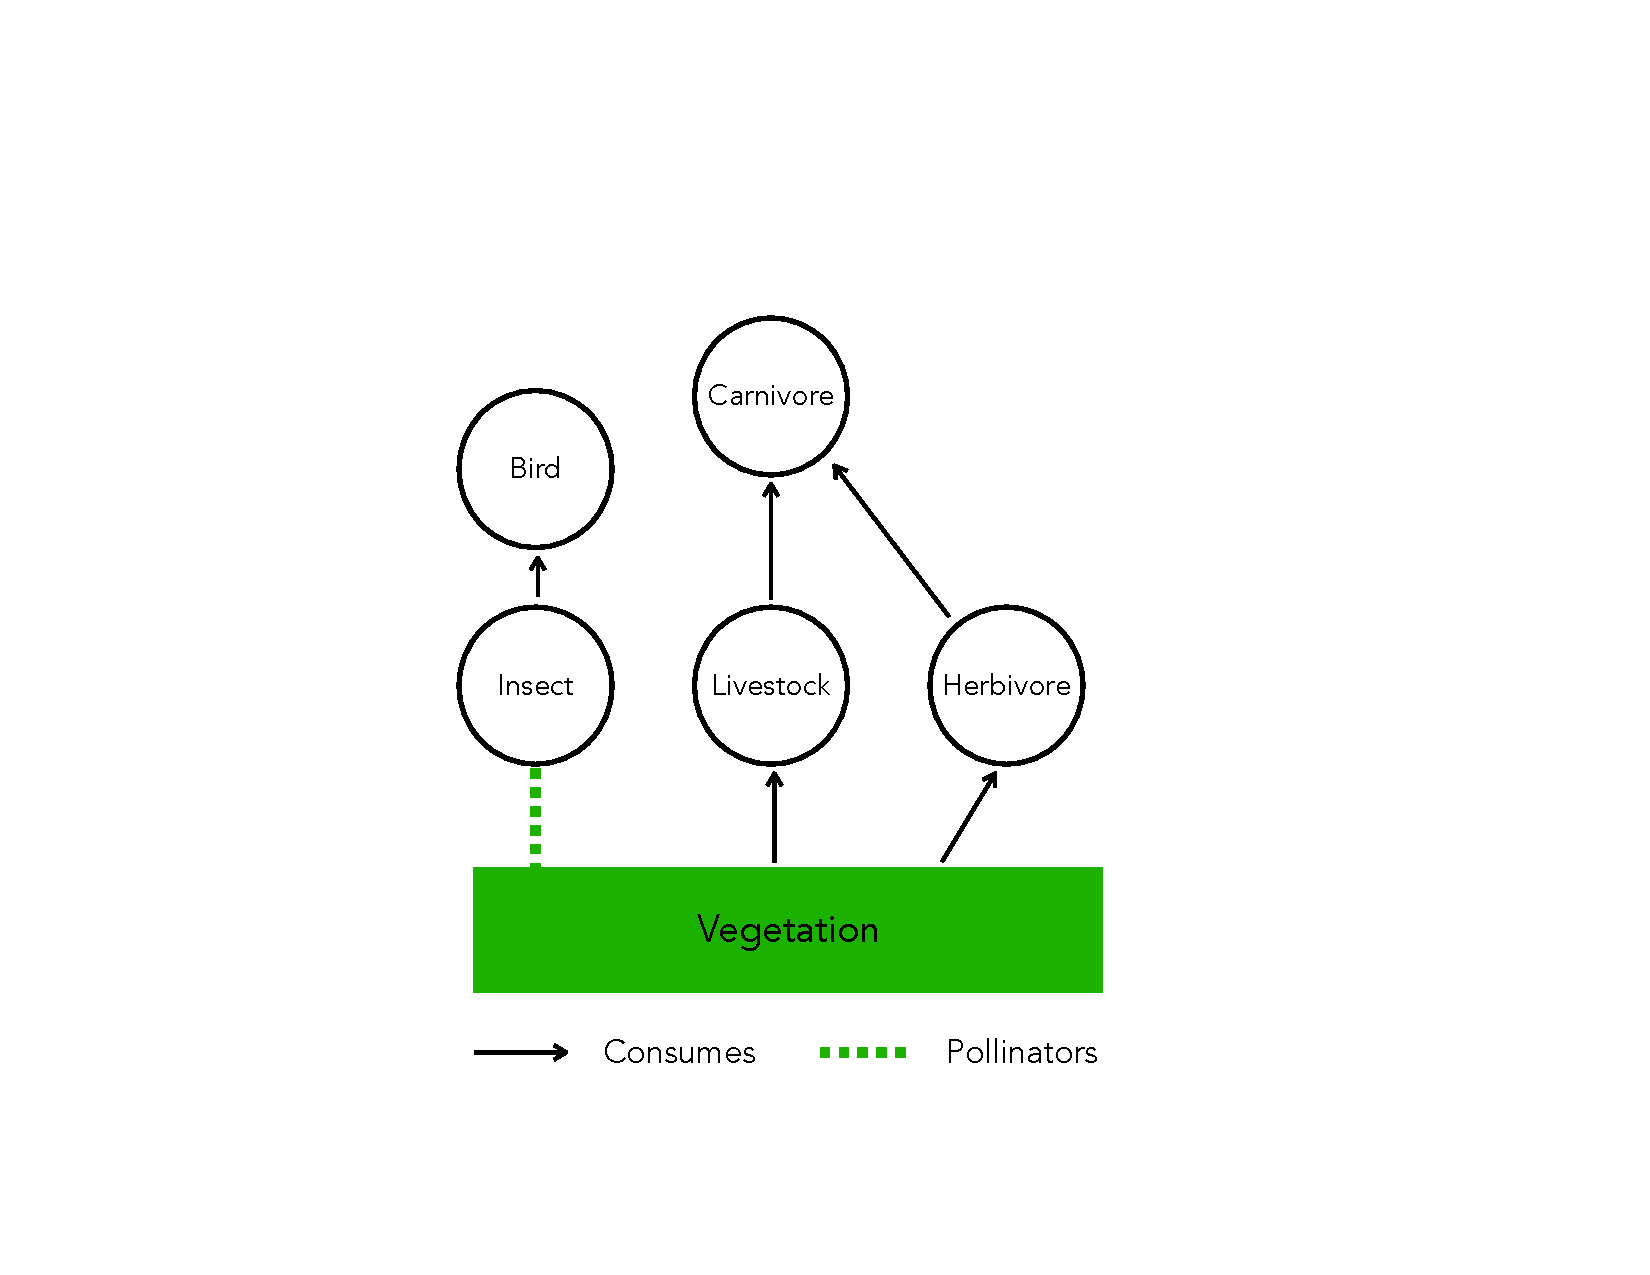
\includegraphics[width=0.375\textwidth]{Figures/TrophicNetwork.pdf}
  \label{fig:TrophicNetwork}
\end{figure}

Non-humans
have a location, ``energy'' they have to move or give to those who consume
them. Livestock are furthermore connected to a landholder, who own them and
the land on which they roam.

\begin{table}[h]
  \caption{\textbf{Non-human animal variables.} All non-human species have
  the share a set of attributes. Predators have an additional attribute, called
\textsc{catch\_radius}, specifying how close prey must be in order to catch it.}

  \label{tab:nonhuman}
  \begin{tabular}{cl} \toprule
    variable & description \\ \midrule  
    \textsc{position} & Spatial location of animal \\
    $\Delta$\textsc{energy} & Energy used to live for one time step \\
    \textsc{energy} & Amount of energy animal has left; animal dies when $<0$ \\
    \textsc{species} & Animal species: insect, bird, herbivore, carnivore, or
    livestock \\
    \textsc{landholder} & Pointer to landholder if animal is livestock; \texttt{NULL}
    otherwise \\
    \textsc{catch\_radius} & Distance away for which a prey animal can be caught; \texttt{NULL} for non-predators  \\
    \bottomrule
  \end{tabular} 
\end{table}

\subsection{Model dynamics}


\section{Results}

\begin{figure}
  \caption{\textbf{Spatial time series of fence construction.} Fences (pink
  polygon overlays) are constructed over time in response to carnivore
  predation of livestock and encroachment by other herbivores. Vegetation is
  shown in green, with darker cells indicating less vegetation due to consumption
  by livestock and other herbivores. Time $t$ is in months.}
  \centering
  \includegraphics[width=0.9\textwidth]{Figures/fencing_series_10y.pdf}
  \label{fig:fence_series}
\end{figure}


\begin{figure}
  \caption{\textbf{Biodiversity prevalence dynamics.}}
  \centering
    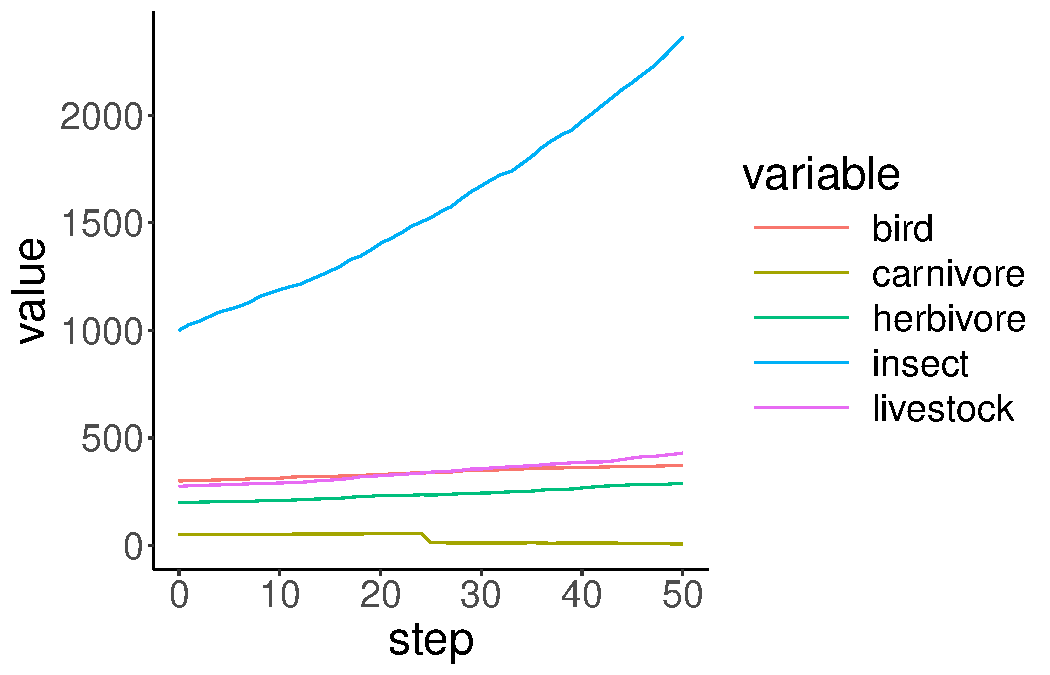
\includegraphics[width=0.7\textwidth]{Figures/prevalence_dynamics.pdf}
  \label{fig:prevalence_dynamics}
\end{figure}


\printbibliography

\end{document}
